\chapter{Head To Toe 2}

% \begin{figure}[H]
%     \centering
%     \includegraphics[width=\textwidth/2]{./Games/EveryChildCanSucceed/Images/EveryChildCanSucceed1CD.png}
%     \caption{Every Child Can Succeed 1 CD}
% \end{figure}

The second of the Head To Toe games published and released by The Lightspan Partnership for the PlayStation 1.

Head To Toe 2 features four video programs:

\begin{itemize}
    \item Standing Tall
    \item Fresh Air
    \item Fueling Up
    \item From Fuel to Waste
\end{itemize}

\clearpage
\newpage

\section{Standing Tall}

\subsection{Audio Summary}

"Standing Tall" focuses on the functions and care of the skeleton, bones and joints.

\subsection{Transcription}

Bob: One, two, three, hi! One, two, three, go! Da da da da da da, da! Swing the other way! Da da da da da da, da! One, two, three, go, hop!

Boy 1: Who turned off the lights?

Bob: We were just playing around with our umbrellas, it was kind of rainy today and everybody brought them in, so we were just having a little fun. Okay everybody, time to put your umbrellas back in the closet. Do you know that you are like an umbrella? I mean, you don't look like an umbrella, but well, here's what I mean. An umbrella is just a round piece of cloth that's kind of loose and floppy, and it gets its shape because on the inside there are some stiff wires, and these wires stretch the cloth out and give the umbrella its umbrella shape. Well, you're the same way. You have soft skin on the outside of your body that covers you all over, and on the inside you have bones. Now you can feel a bone just like this: hold your arm up and squeeze your arm and just feel around here, especially underneath your wrist. Can you feel something hard in there? That hard thing is a bone, and it's like the wires in the umbrella. It's stiff and it's hard and it gives you some shape. Now how many of these bones do you think you have in your body? 50? 87? 100? More than 200? Did any of you guess more than 200? Well, if you did, you're right. That's hard to imagine that we have that many bones inside our body. I'd like you to meet someone who can show us just how many bones we really do have. This is Mr. Bones. Hi, Mr. Bones, nice hat. You ever seen one of these? It's called a skeleton, and a skeleton is a collection of all the bones of an animal or a person who've been put together so that you can see what they look like. Now this skeleton isn't real, it's just made of plastic, but it shows you all of the bones that make up the human body. Now, were you already guessing that this was the skeleton of a human body before I told you that? I mean, look at it. Does it sort of look like a human? There's a head at the top, there are some shoulders, there's two arms with hands, two legs. So a skeleton has the same shape that I do, and that's one of the things that a skeleton does - it gives you your shape. Now here's another skeleton that has a different kind of shape. Where do you think this skeleton came from? It doesn't look like a human person, so what do you think it is? Well, let's look at it. It has four legs. See? One, two, three, four. On the ends of the toes are some sharp claws. There's a head over here at this end that has some long teeth on it, and the back is kind of curved, and then there's a long tail over here. What do you think this skeleton is from? Well, this is from a cat. Kind of looks like a cat, doesn't it, you know when you pet a cat and their back arches up like that? It's about the size of a cat. So a skeleton gives you a shape. I'd like you to meet someone else. Now this is a very unusual skeleton. Kind of looks like a paper plate. Actually, it is a paper plate, and underneath the paper plate is a friend of mine. I'd like you to meet Gertrude the guinea pig. Hi Gertude, come on out, come on out and say hi to everybody. She likes to be scratched right behind the ears just like this, don't you? Can you see how tiny her feet are? Yeah, and she's talking to us too. Look at her little tiny claws and little tiny feet. There, she's pointing them out to us. Gertrude is a small animal, so what do you think her skeleton would look like? Well, I have a guinea pig skeleton here. Here, Gertrude, you just sit right there. That's good girl, and you can watch. Here is a guinea pig's head, and look at the shape of the skeleton head compared to Gertrude's head. Yeah, you agree, don't you? You see how it has the same shape? And look at the front, there's some really strange curved teeth here at the front and some more teeth underneath. And that's one of the nice things about looking at skeletons: you can see what an animal looks like on the inside. You can't tell what Gertrude's teeth look like just by looking at her on the outside like this, can we? Yeah. Here's some other bones from a guinea pig. A little tiny, they're not very big and they're really light. They hardly weigh anything at all, and that's because Gert doesn't weigh very much either. Hey what do you think of thi-

Sam: Hi Bob, what you doing?

Bob: Well hi Sam. I'm just playing with Gertrude the guinea pig. Would you like to meet her?

Sam: Hi, Gertude.

Bob: Yeah, she likes to be petted. And I'm looking at Gertrude's skeleton, or a guinea pig skeleton, and they're really tiny bones, aren't they? They don't weigh very much. Can you imagine an animal that has a really large skeleton?

Sam: Once I saw a skeleton as big as a car.

Bob: As big as a car? You're kidding.

Sam: No, I'm not.

Bob: Where did you see a skeleton as big as a car?

Sam: I'll tell you. I was out with Jody to the museum.

(video plays)

Sam (voice over): She wanted to see the turtles. She really likes turtles, and she has pictures of them in her room and on her book bag.

Sam: Hi, Melissa.

Jody: Hi, Melissa. I'm just a turtle person.

Sam (voice over): But before we even got to the turtle room\dots

Jody: Wow!

Sam: A Chasmosaurus!

Jody: How do you know?

Sam: Well the shape of a Chasmosaurus. See the big head with the pointy things on it?

Jody: He's so cute.

Sam (voice over): Also at this museum, they have a place where you can dig for dinosaur bones, because that's where people find dinosaur bones, in the ground.

Jody: I found something!

Sam: Me too!

Jody: I know mine is!

Sam: What?

Jody: Hmm\dots Definitely a [footprint].

Sam: Are you sure?

Jody: No, I'm definitely just guessing

Sam (voice over): We had so much fun looking at the bones, we forgot to see the turtles.

(next scene)

Arnell: Guess what I have? I'll give you a hint: it's an animal. I'll give you another hint: it's the kind that doesn't have any bones. Give up? A worm. Worms are kind of floppy-like, and you can almost tell they don't have any bones. They aren't stiff and they can't stand up. Do you ever wonder what it would feel like if you didn't have any bones?

(back to house)

Bob: Well, Mr. Bones can show us all about joints. Let's start with the elbow joint that I had in my arm. Here's his arm, and you can see that there's a really stiff bone up here - a big one, that's the top part of the arm, and there are some really stiff bones down here - that's the bottom part of the arm, and where they join together, that's the joint. That's the part that moves and that's the part that bends at the elbow so that we can do this. Now there are lots of other joints in Mr. Bones here. Now, Arnell, what part of your body did you say you could move?

Arnell: A neck.

Bob: Your neck? Well, look at Mr. Bone's neck - he's got all kinds of bones up here, and where they join, he can move his neck around. And Louisa, what did you move?

Louisa: My hand.

Bob: Your hand? Can we find his hand? There it is. Sure, and his hand can go up and down like that. How's your hand move? That's right, and that's where some bones come together so that they can move. And Sam, what did you move?

Sam: I said I could bend my fingers.

Bob: Let's look at Mr. Bone's fingers. Yeah, see, you move your fingers and where these bones come together, they move, and those are joints. Even though the bones themselves are very stiff, the joints are where they can bend, and that's so that we can bend. Can you find any other joints in Mr. Bone's body? What other joint -

Louisa: His knees.

Bob: His knees, right, yeah. Look, he's got two knees. Where's your knee? Where's your knee? That's this one down here, right? Big joint right there. What does this part of the body right here remind you of?

Arnell: A cage.

Bob: A cage. That's right, Arnell, and that's because it is a cage, and we call it the rib cage - all these bones right here. And inside the cage is one of these. You know what this is? What it looks like? You know?

Louisa: A heart.

Bob: It looks like a heart. And the human heart looks something like this, and it's very soft and very delicate, and it could be hurt. So to protect it, it goes inside the cage. So we're going to give Mr. Bones a heart, and your heart sits right about there. And there are some other things in there like lungs, and they're very soft, and so they're protected by these bones of the rib cage. Can you feel your rib cage? Just feel down your side. Just tap it a little bit, and you can feel those hard bones that protect your heart and your other organs. And there's one other part up here at the top. Why do you think we have a hard bone at the top of our head?

Children Together: Cuz you have a brain.

Bob: We all have brains, right? And brains are very soft too, and we don't want to hurt them, so they're protected inside the skull. And if you just tap your head just very lightly, you can feel that hard bone that's in there. So our bones also give us protection.

(doorbell rings)

Children Together: I'll get it.

Sam: Hi, Janice.

Children Together: Hi, Janice!

Janice: Hi, guys. Boy, am I having a bad day.

Bob: Hi, Janice.

Janice: Hi, Bob.

Louisa: Janice, what happened to your arm?

Janice: I broke it.

Arnell: How?

Janice: Skating, that's how.

Bob: Janice, don't you wear a helmet and elbow pads and knee pads when you skate?

Janice: Well, usually I do, but this time I was in a hurry and the sidewalk was wet and I fell real hard and I broke my arm.

Sam: Did it hurt?

Janice: A little at first, but now it's okay.

Bob: Well, that's why we have to think about safety, cuz even though our bones protect us, we have to protect our bones as well.

(video plays)

Male singer: Oh, when you think about your bones, where do you begin? Cuz your bones do more than give you a place to hang your skin. They help to keep your insides safe and sound. They help you walk, sit, stand, and run. And when you put 'em all together, what do you have? Your skeleton. Everybody gets a set. It's the only set that you get. The only thing you need to do is take care of your bones and they'll take care of you. Want to take care of your bones? It's not hard to do. Just remember these simple things that we've been showing you. We got a question for you before we're done. Did you think your bones could be so much fun? And did you ever really think you know this much about your skeleton? Everybody gets a set. It's the only set that you get. The only thing you need to do is -

Female singer: Take care of your bones and they'll take care of you.

Male singer: Just take care of your bones, they'll take care of you.

(Back to house)

Bob: Here are three different drinks. Which one do you think is best for your bones? We have apple juice, we have Cola, and we have milk. Which one is best for your bones? Hmm. Answer is\dots

Janice: Milk.

Bob: Answer is\dots Right, milk. Sure, lots of people tell you that milk's good for you, but they never tell you why. Well, milk is good. Actually, milk is great, and that's because milk helps your bones grow. It makes them strong and keeps them healthy. Actually, there are some other foods that are good for your bones too. I have some over here in the fridge. One of them is cheese, and that's because cheese is made from milk. And the other one, I have one more here. This is\dots Let's see, it's in here somewhere. Oh, there it is. Yogurt. Yogurt's made from milk too. And it's\dots Hey, what happened to the cheese and milk? Sam, what are you doing down there?

Sam: I'm just having some bone food.

Bob: Bone food?

Sam: Ah, delicious!

Bob: Well, why don't you just share your bone food with Arnell and Louisa?

Sam: Come on, you guys!

Bob: Let's have some bone food here, and have a little party. Okay, here you are, Louisa. You could have some bone food.

Louisa: Thank you, Bob.

Bob: You're welcome. And here you are. Have some for your arm now, you need a little extra there.

Janice: Thank you.

Bob: You're welcome. Here you are, Anell. You have some bone food.

Arnell: Thank you.

Bob: You're welcome. Everybody eat up, enjoy your bone food. Food is important if you want your bones to be healthy, but there's one more thing that your bones need. They need exercise. So running, jumping, playing - these are all activities that help your bones stay strong and stay healthy.

(video plays)

Bob (voice over): Your bones are strong and stiff. Your bones are all connected - that's called your skeleton. Your skeleton protects you, especially your rib cage and your skull. Exercise is great for your bones, but you also need to protect them sometimes, and eat and drink the right foods like milk and cheese.

(Back to house)

Sam: There, finished.

Bob: So what did you write, Sam?

Sam: I wrote, 'Dear Janice, when I told you give me a break, I didn't mean this. Signed, your arm.'

Everyone Together: Oh\dots

Janice: Thanks, Sam.

\subsection{Credits}

Special Thanks to: The Children's Museum of Indianapolis, Wayport Pet Supply;
Models Donated by: Frey Scientific Inc, Denoyer-Geppert Science Company;

\section{Fresh Air}

\subsection{Audio Summary}

"Fresh Air" describes how the lungs get oxygen, and how to keep the lungs healthy.

\subsection{Transcription}

Bob: Well, that looks like fun, doesn't it? Would any of you like to walk in space?

Chao: Yeah!

Naomi: Absolutely!

Jody: You don't really walk, you just float.

Bob: Boy, I'd sure like to be up there floating around and having fun in space. But I have a question: why do astronauts have to wear those space suits all the time? Does anybody know?

Chao: I do! Because there isn't any air in outer space.

Bob: But why is air so important?

Naomi: Because they have air in their space suits so they can breathe.

Bob: Oh, so they can breathe. Hm, well that's very interesting. You know, I know of another place where there isn't any air, and when people go there, they have to wear special equipment. They have to wear a special mask so that they can breathe. Any idea where it might be?

Children Together: No.

Bob: Let's watch and find out.

(video plays)

Bob (voice over): When you go swimming, you know that you can't stay underwater for very long. You have to hold your breath because there's no air to breathe underwater, and people need air to breathe and to live. So if you want to spend a long time underwater, you have to do what these divers do. You have to bring some air with you. They have air in those tanks on their backs.

(Back to house)

Bob: So when people go underwater or when they go into space, or even if you're just running around the house, you need air to breathe. And air is kind of mysterious stuff, isn't it? I mean, you can't see it, you can't feel it. Although (if you) do this, just run your hand up and down really fast, can you sort of feel it going through your fingers? You can feel it a little bit. Air is actually real stuff. We can sort of see what air is like - this bag doesn't have anything in it right now, right? Okay, so let's fill it up with air, and we'll get the bag really full of air. And look, now it feels like there's something in there. Can you feel that?

Naomi: Yeah, it feels really squishy.

Bob: But you can push on it - there's something in it. Air is real stuff. I mean, airplanes fly in it, and birds fly in it, and yet inside the bag, it looks like there's nothing at all: just air. And we need air to breathe, and you're breathing right now, and so are you. Now when you do breathe, where does the air go into your body?

Jody: Your nose.

Bob: To your nose.

Chao: To my mouth.

Jody: Your nose!

Chao: Your mouth!

Bob: Hm, we seem to have a little argument here. Your nose, your mouth. I wonder which it is. Let's do a little experiment. Put your hands over your mouth like this, really tight. Okay, now just breathe while you're doing that. Where's the air going?

Jody: Through my nose.

Bob: Through your nose. And if you do it really fast, you can actually hear it going in and out. Okay, now try this. Take your finger and put it over your nose like this. Pinch so that - okay\dots Now breathe again. Where's the air going this time?

Chao: Through my mouth.

Bob: Through your mouth.

Naomi: So you're both right!

Bob: Yeah, you're both right. The air goes into your nose or into your mouth, or both. And actually, it's a good thing that it can, because sometimes when you have a cold, your nose gets all stuffed up and you can't breathe through your nose, so it's a good thing that you can still breathe through your mouth. Well, if you need to breathe the air in through your nose and your mouth, where does it go then? Where does it go inside your body? Want to find out? Everybody up! Let's try this, and you can try this as well. Put your hands on your side, so, put them like this, okay. Just feel your chest. Now take in a really deep breath. You ready? One, two, three, in! Hold it. You feel how your chest gets bigger when you do that? Okay, now let it out. And when you let it out, your chest gets smaller. Okay, breathe in one more time. When you breathe in like this, all the way in, the air goes in through your nose and mouth and into two large bags that are inside your chest called your lungs. Would you like to see how your lungs work? Come on, I'll show you how your lungs actually do that.

Chao: Can we breathe out yet?

Bob: Oh yes, yes, yes, you can breathe out. You can breathe out now. Okay, don't hold it in like that. Now let's see how your lungs really work inside your chest. Come on.

(move to another room)

Bob: Now if you could see inside your chest, that's what your lungs look like. These two pink bags right here. And when you breathe, these bags fill up with air. And the red thing that's in the middle, that's your heart. So your lungs kind of wrap around your heart like that. Now the way they work is something like, well, it's sort of like this. Naomi, can you blow that balloon up? When you breathe in, your lungs get bigger like the balloon because they fill with air. And then let it go. When you breathe out, the air goes out and your lungs get smaller. So your lungs are just like two balloons that are in your chest like this, and you have a tube that comes up your throat, and it ends up at your nose and your mouth. And that's where you breathe in and out. Now let's have a closer look. Since this is a model, I can take it apart, so let's take this lung apart. There we are. And I'll take the heart out so that we can see this a little better. There we have our two lungs, and here's the tube that comes down your throat, and then see how it splits here? One goes to one lung, one goes to the other lung, and then it keeps splitting. It splits again here, and then it splits again there, and it keeps going down, and these tubes carry the air to every part of your lungs. And then, see these little tiny spots there? You can just barely see them. The tubes lead to what are called air sacs, and they do just what their name means: they take in and they fill up with air. Let's have a closer look at the air sacs.

(video plays)

Bob (voice over): As it fills up with air, an air sac does a wonderful thing: iIt takes something out of the air, a special gas, and it puts that special gas into your blood.

(Back to house)

Bob: What is this special gas? Well, first we have to understand that air is actually made up of lots of different things. It's just a swirl of all these different invisible gases. But your body only needs one of them, and that one's called oxygen. Now let me spell that for you.

Jody: I can spell it!

Bob: You can spell oxygen? That's a pretty hard word.

Jody: Give me a break. O-X-Y-G-E-N. Oxygen!

Bob: Whoa! Let's hear it for Jody! Oxygen - that's what your body needs. But it's only one part of the air. So your lungs do a very important job: they take just the oxygen out of the air so that your body can use it.

(video plays)

Bob (voice over): When you breathe in, your air sacs take just the oxygen out of the air and put it into your blood. Your blood takes the oxygen to every part of your body. But something else happens: after your body uses the oxygen, well, you have inside of you a lot of gases that you didn't use. We call that used air. How do we get rid of used air?

(Back to house)

Bob: You breathe out. So come on, let's get rid of some used air! When you breathe out, your body is getting rid of gases that it just doesn't use. So it's oxygen in, used air out.

(video plays)

Male singer: Be glad that you breathe out your air, it's the toot on the flute and the trumpet. Be glad you can blow through your mouth when balloons need to be blown up. And be glad you can whistle and sing, every sneeze is a reason for rejoicing. Be glad that you breathe out your air, with every pump you have the [stump] to make excitement. Be glad that you breathe out your air, be glad when you're huffing and puffing. Be glad that there's air everywhere, 'cause it lets you giggle and laugh. Be glad that you know that there's air, you don't see it, but you know it's always with you. Be glad that there's air everywhere, with every pump you have the [stump] to make excitement.

(Back to house)

Bob: So we know what your lungs like: pure, clean oxygen. But are there things that your lungs don't like? And how do you know if your lungs don't feel right? Well, you cough. Excuse me. Have you ever done that? When you cough, your lungs might be telling you, 'Hey, there's something in the air we just don't like.' Now let me show you some things, and you tell me which of these things would make you cough.

(video plays)

Bob (voice over): Would this make you cough? Probably not. What if you breathed in that smoke? How about this? Would your lungs like this? Do you think you'd be coughing here? What about cigarette smoke? Does that ever make you cough?

(Back to house)

Bob: Smoke makes you cough, doesn't it? And it doesn't matter if it's smoke from burning leaves, a cigarette, or even a smokestack, your lungs just don't like it. And you can probably guess why: your lungs like oxygen, right? Well the smoke prevents that oxygen from getting in, so one of the ways to keep your lungs healthy is to just stay away from smoke. But what if you can't stay away from smoke? What if your job takes you near fire? You know who I'm talking about. Hi, Mr. Bones! Nice hat! Firefighters are around smoke all the time. So how do you think they prevent that smoke from getting into their lungs? Well, Chao's neighbor is a firefighter, and recently he went to visit her.

(video plays)

Firefighter: So how are you doing today, Chao?

Chao: Fine.

Firefighter: That's good. You've come to the firehouse today to find out how firefighters keep their lungs safe in a building fire?

Chao: Uh-huh.

Firefighter: That's a very good question. We have a special piece of equipment called a self-contained breathing apparatus. We call them the SCBA for short.

Chao: It looks like a scuba diver's tank.

Firefighter: That's exactly what it is. But this one you don't use underneath the water: this is for when you're on the ground. We use this to go into building fires because there are so many poisonous gases from the things that are burning in the fire that we can't breathe that air. There's no oxygen in it, so we take our own air in this bottle. There's about 30 minutes of air in here. The air comes out of the tube and it goes into the mask, okay. Would you like to try it on?

Chao: Sure.

Firefighter: Okay, be careful. It's kind of heavy.

Chao: Whoa, this is heavy!

Firefighter: Okay, let me help you hold it. Okay, first thing you have to do is make sure that it's on. Okay. Then you put the mask over your face and you breathe it in. There's a plastic shield on there so you can see what you're doing. You feel the air?

Chao: Uh-huh.

Firefighter: See, this is clean air. It's not the air that you're going to breathe in a house that is burning.

Chao: This feels funny.

Firefighter: Let's turn it off.

(Next scene)

Chao (voice over): People need air. You breathe through your nose and your mouth. The air goes down an air pipe and into your lungs, and when you breathe in, your lungs get bigger. Inside of your lungs are tiny sacs called air sacs. They take the oxygen out of the air and put it into your blood. When you breathe out, you're getting rid of used air. You breathe out when you talk and whistle. Your lungs don't like smoke. Stay away from smoke if you want your lungs to stay healthy.

(Back to house)

Bob: And nice fresh fruit! Here's one more thing to think about when it comes to your lungs. I'm sure your parents have told you that this is not a toy. Since we've been thinking about our lungs today, I'm sure you can see why this is a dangerous thing to play with. Oxygen does not go through plastic, so if you put this bag over your head, the oxygen cannot get into your lungs. That's why it's dangerous. It's also dangerous to put yourself into a small closed trunk or a closed refrigerator. There just may not be enough oxygen in there for you to breathe. By the way, there's something else we can do with the air that's in our lungs. We can use it to sing. It's Jody's birthday today.

Everyone: Happy birthday to you!

\subsection{Credits}

Models Donated by: Frey Scientific Inc, Denoyer-Geppert Science Company;
Footage Provided by: General Learning Video, SeaWorld of Florida;
Special Thanks to: Indianapolis Fire Department, NASA;

\section{Fueling Up}

\subsection{Audio Summary}

Fueling Up shows how the body digests food and uses it for fuel. It also talks about the five food groups, and importance of foods to maintain good health.

\subsection{Transcription}

Arnell: These are good.

Diego: Mmm\dots

Sam: Taada!

Arnell: Who are you supposed to be?

Sam: I am Sam the magician, and I will now make something disappear. Watch carefully. Nothing up my sleeves\dots and abracadabra! It disappeared. I am amazing!

Diego: That's not magic.

Sam: Well then where did it go? Do you know?

Bob: Do you know where it went? What happens to food after you swallow it? Does it just disappear like magic?

Arnell: Oh, I know where it goes. Food goes down to your stomach!

Bob: Well, you're right Arnell. Food does go to your stomach, but how does it get there and what happens to it after it's in your stomach?

Arnell: I don't know.

Bob: Well, why don't we find out? Let's think about the amazing trip that food makes when it's inside your body. Come on, I'll show you.

(move to another room)

Bob: Isn't this neat?

Children Together: Yeah!

Bob: This is what it would look like if you could see inside your body. And here are the organs that help you digest food. Uh, hmm\dots There seems to be something missing over here. We don't have a head and we need a head because that's where the trip that the food takes begins. Who wants to be the head?

Diego: I will!

Bob: Okay Diego, come on back. You can be the head. Good! Now we have a nice head, get right in there. So uh, Diego, uh, how you doing today? Say you're hungry.

Diego: I'm hungry.

Bob: Hungry, huh? Hm, what's it feel like to be hungry?

Diego: Um, my stomach is growling and I don't have any energy and all I can think of is getting some food.

Bob: Excellent. Isn't it amazing how your body tells you that it needs food? You can actually feel it. Uh, so Diego, would you like a muffin?

Diego: Yes, please.

Bob: Coming right up. Here we are. This is the beginning of a very long trip for this muffin. Now where does it go?

Arnell and Sam: In his mouth!

Bob: In the mouth. Open wide! Ah! Well, we're already seeing the first thing that happens to the food. You chew it up. Now when you chew, your teeth act like knives and they actually cut the food into little tiny pieces. But there's something else that happens inside your mouth. Your mouth is wet and that liquid that's in your mouth helps make the food soft. So we'll just add a little bit of liquid here. So your teeth cut it into little pieces and the liquid in your mouth makes it soft until it looks, well, something like that. And once it looks like this, you're ready to swallow. Have you swallowed your muffin Diego?

Diego: Yes.

Bob: Okay, when you swallow it goes down your throat. So right now these little pieces of food go down a tube that's inside your throat and when you swallow they go down and down and down until they end up inside\dots Arnell, what?

Arnell: In your stomach!

Bob: Right, and there's your stomach right there and that's where the food goes. But the trip isn't over yet because something else happens inside your stomach. Your stomach also has liquid in it, so we add a little bit more to our muffin. And your stomach can move, and it does something like your teeth, it sort of grinds the food up into even smaller pieces. Hm, like this. So that eventually the muffin doesn't look like a muffin anymore, it looks something like\dots Eugh.

Arnell: Eugh, what is that goop?

Sam: Yuck!

Bob: Well that goop, that goop is what's inside your stomach right now. The liquid has made it soft, it's been chewed into very, very tiny pieces. But the trip isn't over yet. There's still one more place that it goes, and that's into your intestines.

Arnell: Yuck!

Bob: If you could look at your intestine in a microscope, you'd see that it actually has millions of tiny little holes in it. So when the food goes through the tube, some of the food slips out through those holes. So that means that some of the food that you've eaten comes out here and some of it comes out over here, some over here, slipping out through those millions of tiny little holes. Now here's the amazing part. Once the food goes out through those holes in the intestine, where do you think it goes? Into your blood.

Sam: Your blood?

Bob: Uh-huh. The food that you've eaten goes into your blood. So Arnell and Sam, would you like to take these red pens here and show us just where blood goes in your body? Just draw it right on Diego's body there.

Arnell: Your blood goes to your heart, then some to your arms and hands and fingers.

Sam: Some blood goes down your legs and to your feet.

Diego: Don't forget my brain.

Arnell and Sam: Okay.

Arnell: Here's the blood going to your brain.

Bob: Your blood goes almost everywhere in your body, and in your blood are those tiny pieces of food. And that's how your body gets its food. When you eat, your teeth mash the food into little pieces, your stomach turns it into a liquid so it can go into your intestine, into your blood, and flow throughout your entire body. And that happens every time you eat.

(skip to another room)

Bob: Oranges. Hm. What if all you ever wanted to eat were oranges, and you had oranges for breakfast, oranges for lunch, for a snack you have oranges, oranges for dinner. You'd get tired of oranges pretty fast, wouldn't you? And at the same time, your body would not be getting everything it needs to stay healthy. I mean, oranges are good for you, but your body needs different kinds of food so that it can grow, so that you can have energy. Energy to ride your bicycle, run upstairs, and move all the parts of your body. But how do you know which are the right kinds of food to eat? Well, the kids can help us find out. Arnell, Sam, Diego, come over here. Hi guys.

Children Together: Hi Bob!

Arnell: We made the basket -

Sam: - for the five food groups.

Bob: That's great. What's the food groups Sam?

Sam: It's a lot of different foods that are alike, like milk. That's all the foods that come from milk, like yogurt and cheese and ice cream.

Arnell: Milk are good for your bones and teeth.

Sam: And vegetables. Vegetables come from plants like beans and lettuce and carrots.

Diego: Veggies are good for your blood and your skin and your eyes.

Bob: Oh, I see. So by eating different foods, the parts of your body get everything they need to stay healthy.

Sam: Correct.

Bob: Ah, well how many different food groups are there?

Sam: Five. Meat and milk and fruit and vegetables and bread.

Bob: Bread, huh? Hm\dots What's in the bread group, Arnell?

Arnell: Oh, things like bread of course, and cereal and rice and noodles.

Bob: Great. Well, you guys did an excellent job. Now here's what I'd like you to do now. You see all this food I have over here?

Arnell: Yeah.

Sam: Yeah.

Bob: Okay. I wonder which types of food go into the different groups. Do you think that you could sort all this food and put them into the different baskets so they're in the right groups?

Children Together: Sure, no problem. Piece of cake.

Bob: All right. Yeah, well, there's a catch to this. There's a catch to this. Do you think you could do all of that in less than 30 seconds?

Children Together: Huddle! Yeah, we can do it!

Bob: Okay, are you ready? Go!

Children Individually: Chicken, meat. Peas, vegetable. Carrot, vegetable. Raisin bread, bread. Potato, vegetables. [Raising bread], fruit.

Bob: Five seconds.

Children Individually: [Fish], meat.

Bob: All right, congratulations! You're finished. Under 30 seconds. Now let's see what ended up in each basket.

Sam: In milk we have yogurt and ice cream and milk.

Arnell: And in meat we have chicken, fish, and peanut butter.

Diego: And in vegetables we have peas and carrots and lettuce.

Sam: And in fruit we have apples, oranges, and bananas and a loaf of raisin bread.

Arnell: And in bread we have crackers and a loaf of raisin bread.

Bob: Perfect! What's neat is that you can see that there really are five different groups of food. So if you want to stay healthy, just make sure that you eat food from all five groups every day, and that way you're sure that your body has everything that it needs to be healthy and grow strong. Our friend Chao learned about the five food groups earlier this week. He went to a place where food comes from. He visited a farm.

(video plays)

Male Farmer: So we grow most everything we eat right here on the farm.

Chao: You never go to the grocery store?

Male Farmer: We go to the grocery store sometimes, but most everything we eat is right here on the farm.

Chao: I don't see the five food groups.

Male Farmer: I tell you what, you're going to be here on the farm all day. You look and see if you can find the five food groups.

Chao: I will.

Male Farmer: We're going to see the first one right in here.

(move to cow barn)

Male Farmer: Okay, Chow, we got the cows in. Let's see if you can't find one of the five food groups in here. Which one's that?

Chao: Milk!

Male Farmer: Right! How would you like to milk?

Chao: Sure.

Male Farmer: Grab a hold of the top and squeeze down. That-a-way. Here, you sit down and milk the cow!

Chao: This is fun.

Male Farmer: Yeah! There you go, now you're getting milk from the cow! We use milk on our cereal, we make butter out of milk, we make cheese out of milk.

Chao: And ice cream?

Male Farmer: And ice cream.

(move to apple orchard)

Male Farmer: These look good, Chao. See if you can find one.

Chao: Yeah, these look really pretty.

Male Farmer: Good, let's go [wash] 'em.

(move to sheep pen)

(move to pumpkin patch)

Female Farmer: This is our pumpkin patch, Chao. We have a few this year, not quite as many as what I'd like, but we have some pretty ones in there. Would you like one?

Chao: Yeah!

Female Farmer: Why don't you take this one home?

Chao: Thanks.

Female Farmer: Well, you're welcome.

(move to pepper field)

Female Farmer: Chao, I think there's nice big pepper down there. Oh yeah, that's a nice one!

(move to tomato plants)

Female Farmer: Chao, here's some Better Boy tomatoes. Would you like to have some of those for your basket?

Chao: Sure.

Female Farmer: They're just really ripe, aren't they?

Chao: Uh huh. I never knew tomato plants could get this big.

Female Farmer: Well these sure did.

(move to chicken coop)

(move to green bean field)

Chao: Ah, green beans. The vegetable group.

Female Farmer: They sure are.

(move to sitting area)

Chao: I like to be a farmer. You know why?

Male Farmer: Why?

Chao: Because it's just about the best tasting job you can have!

Male Farmer: *laughs*

(back to house)

Sam: For my next trick, I'll turn this apple into a liquid.

Arnell: And for my next trick, I will turn this carrot into a liquid.

Diego: And for my next trick, I'm going to turn this sandwich into a liquid.

Bob: What happens to food inside your body isn't magic, but it sure is amazing. And it's good too, isn't it? Mm, let's eat.

Arnell: Okay, pass over the sandwich.

Everyone: *laughs*

\subsection{Credits}

Special Thanks to: SeaWorld, Merrill and Larene Scott Farms;
Models Donated by: Frey Scientific Inc, Denoyer-Geppert Science Company;

\section{From Fuel to Waste}

\subsection{Audio Summary}

From Fuel to Waste looks at the way your body makes and disposes of solid and liquid waste.

\subsection{Transcription}

Chao: Yeah, get that one. Right there, yeah.

Naomi: Good!

Chao: You got it!

Naomi: Oh, uh, hi. Um\dots

Chao: What?

Naomi: Uh, the show started?

Chao: Oh, hi. Where's Bob?

Naomi: Uh, Bob's not here at the moment.

Chao: Where did he go?

Sarah: Bob had to go to the bathroom.

Chao and Naomi: *laughs*

Bob: Ah yes, hi everybody! What's so funny?

Naomi: Uh, Bob, the show started.

Bob: The show? Oh, hi. Uh, sorry I wasn't here earlier. I uh, well actually I was here earlier but then I had to uh\dots I had to go uh\dots

Sarah: You had to go to the bathroom.

Bob: Well, thanks for telling everybody, Sarah.

Sarah: You're welcome!

Bob: Oh well. That happens, doesn't it? Couple of times every day you have to stop whatever you're doing and go to the bathroom. Well it's nothing to be embarrassed about really, everybody does it. And when you go to the bathroom, your body's actually doing something very important. Well, I guess uh, today's a good day to think about why we have to go to the bathroom. And I know a good place to start. Some of you may have seen an earlier program where we talked about what happens when you eat something.

Chao: I saw that show!

Bob: Oh, that's great, Chao. Maybe you saw Diego eating a muffin? How'd you like to tell us and remind us what happens after you do eat something?

Chao: Sure, that's easy.

(video plays)

Chao (voice over):The first thing you do is chew. Your teeth break food into little pieces, and the liquid in your mouth makes it soft. Then you swallow. The food goes down your long tube to your stomach. Your stomach mashes it and adds liquid, and soon your food is turned into a soupy liquid. It looks like this. Then it goes into another long tube. That's your intestine. It has a lot of tiny holes, and little bits of food go through the holes and into your blood.

(back to house)

Bob: Thanks, Chao, that was great! Well, our program told us what happens to food that's inside your body, but it left out one very important thing.

Children Together: What?

Bob: Come on, I'll show you.

(move to another room)

Bob: Let's do an experiment to show what happens to food when it's in your intestine. Here's a bowl, and over the top of the bowl there is a piece of cloth, and can you see how the cloth has some holes in it? Now those holes are like the holes in your intestine. Now these holes are a lot bigger than the real holes, but that's just so that we can see it. Now when the food goes into your intestine, it goes through the holes and it goes into your blood. Well, let's get some food here. Before it gets to the intestine, it's in your stomach. So here's what used to be a muffin inside our stomach here, and let's suppose you're really hungry, you want to have another one. So Naomi, you want to take this muffin and just grind it up there inside the stomach? Now your stomach adds fluids to that food to help break it down. Hello, Bird!

Bird: Hi, Bob!

Bob: So we'll just add a little bit of fluid here. And then your stomach churns that food around so that it'll break it down even further. So you want to churn up the stomach there. Ah, there it goes, and turns our muffin into a nice sloppy goop. Hm. Okay, now it goes into the intestine. So let's see what happens when it gets to the intestine wall. Naomi, just pour it right on through the cloth there and let's see what happens. Hmm\dots

Naomi: Ew!

Bob: So what happened?

Naomi: All of it didn't go through.

Bob: That's right. Look carefully, you can see that in the bottom of the bowl, some of it did go through, and that liquid that does go through goes into your blood, and then that goes through your whole body, and that's how your body gets food. But your body doesn't use all of the food that you eat. Now we have a name for that. That's called waste. And because your body doesn't use the waste, it has to get rid of it somehow.

Sarah: That's why we go to the bathroom!

Bob: That's right, Sarah. That's why we go to the bathroom. Since your body doesn't use all of the food that we eat, it has to get rid of the waste. And to show you just how it does that, let's go to a model. It's just over here.

(move to another room)

Bob: This is a model of what the inside of your body looks like. Say hi to Kathy!

Children Together: Hi, Kathy!

Bob: Now this part down here, that's where the food goes after you eat it. It's the soft part of your tummy. Can you feel this part right here? Feel how it's kind of soft down there? Yeah, that's this part here. So after you eat the food, it goes in your mouth, down the throat, and into this kind of baggy-looking thing. What do you think that is?

Sarah: A stomach!

Bob: That's right, that's your stomach, and that's where the food is turned into that goop that we had before, and then it goes into this long tube down here. We call that the small intestine, and that's the tube that's as long as this room, and it's all been stuffed up in there, so some of the food goes through the little tiny holes into the blood, and then the stuff that doesn't do that, that your body doesn't use, goes all the way through the tube, and that waste goes into this part here. What do you think that's called?

Naomi: The large intestine.

Bob: Yeah, that's right. It's the large intestine because it's larger than the small intestine, and then that waste goes all the way around here, and the large intestine holds on to it until we need to get rid of it.

Sarah: That's when we go to the bathroom!

Bob: That's when we go to the bathroom. That's right.

*doorbell rings*

Children Together: I'll get it! It's Pete!

Pete: Hey, how you doing?

Bob: Hi, Pete! How's it going?

Pete: Hi Bob, fine.

Bob: Good to see you! What brings you to this part of the neighborhood?

Pete: Well, I just thought I'd stop by and see what you all were thinking about today.

Sarah: We're going to the bathroom!

Pete: Excuse me?

Bob: Um, no, we're uh, we're thinking about how your body gets rid of food that it doesn't use.

Pete: Amazing! I can't believe this, but I once wrote a song about that very subject.

Bob: You did?

Pete: Most people write about love or the moon. I wrote a song about waste.

Bob: Wow! Well, uh, can we hear the song?

Children Together: Yeah!

Pete: Hm, twist my arm, maybe. Okay, I'll do it.

Bob: Oh wow! Okay.

Pete: Uh, you want to play along with me Bob?

Bob: Yeah sure, sure.

Pete: [I mean, you] play guitar.

Bob: Yeah okay, I'll try to follow you here, see if we can make this happen.

Pete: Let's see, it's been a while. Let me see if I can remember this.

Bob: Okay.

Pete (singing): When you have a meal, you sometimes feel you can eat every bit of the food. But when the eating starts, you always find parts, that aren't supposed to be chewed. There's always something left over, the part that you don't eat. Like the stem and the pip and the [inaudible], and the bone in the middle of the meat. Yes there's always something left over that sits there in a clump. So you put in a can and then the garbage man takes it to the dump. Yes you put in a can and then the garbage man takes it to the dump. Now after you eat, and you're feeling real neat, your intestines have work to do. But soon you feel, 'hey part of that meal is moving all the way through'. Cus there's always something left over, the part you don't digest. Your bodies use only part of the food, and leave behind the rest. Yes there's always something left over that sits there in a glop. And that's when you, 'I've got to go', and the bathroom's your next stop. Help me now guys. And that's when you, 'I've got to go', and the bathroom's your next stop.

Bob: All right!

Children Together: Yay!

Bob: Great song, great song! Pete, that's got to be the silliest, the, well, the most wonderful song I think I've ever heard.

Pete: Well, I'd have to admit it's probably is the best song I've ever written about waste.

Bob: Well, you don't hear too many songs about that subject.

Pete: Well, it's getting late. I better be heading out.

Bob: Oh, well, thank you very much for dropping by, Pete. Thanks for the song, that was great!

Pete: Thank you, good to see y'all.

Bob: Okay, bye!

Pete: Bye!

Children Together: Bye!

Pete: Um, by the way Chao, can you tell me where the bathroom is?

Chao: Right around the corner!

Pete: Thank you!

Children Together: Bye Pete!

Pete: Bye!

Children Together: Bye!

Naomi: Great song!

Bob: Well so far we've only been talking about one kind of waste that your body produces. That's the solid waste. But you know that when you go to the bathroom, you also produce a yellow liquid. You know what I mean? Sometimes you just produce the yellow liquid, sometimes just the solid, sometimes it's both. Do you know the name of that liquid? Well, it's called urine, and urine is produced by a different part of your body, but it's also a waste product. Let's go back to Kathy over here. Now here's the small and large intestine. They produce the solid waste. But if we take them out, you can see just behind them there are two other little organs, these purple things here. Those are called your kidneys, and if you want to find out where your kidneys are in your body, just put your hands on your waist like this until your fingers are almost touching behind your back. One kidney is underneath your hand here, and the other kidney is under your other hand back here. Now, after food goes through your blood, the blood needs to be cleaned and get the urine out. Well, that's what the kidneys do. They clean the blood, they produce the urine which is the leftover waste that your body doesn't use, and then it goes down these tubes here and here, and into another part that's called the bladder. And the bladder is really nothing more than just a little bag. It's sort of like this balloon that's filled with liquid. And when that bladder fills up, that's when you need to go to the bathroom. And when you do need to go to the bathroom, the bag empties and you produce the urine. It's kind of neat how your body tells you how you need to go to the bathroom. You suddenly, you just don't feel very comfortable. Well, if you do get that feeling of discomfort, go! It's not good to try to hold it back. So your body produces waste by itself, it gets rid of waste by itself, but you can also help because there are certain foods that actually help your body to get rid of waste. What kinds of foods? Well, Janice went to the store to find out.

(video plays)

Janice: Hi, Janice here! Kid reporter. Today I'm at the grocery store asking people what food helps your body get rid of waste.

(move to inside grocery store)

Janice: Excuse me?

Woman 1: Yes.

Janice: What makes waste?

Woman 1: Doesn't everything make waste?

(move to another part of the store)

Janice: Can you tell me what makes waste?

Woman 2: Well, gee, I never thought about that before. Have you ever thought about that before?

Man 1: No, I haven't thought about that before.

(move to another part of the store)

Janice: Excuse me, can you tell me what makes waste?

Tiffany: That's easy! We learned it in school. I'll show you! Dad, I'll be back. I'm going to be on TV! Hi, Mom!

(move to another part of the store)

Janice: Oh, and by the way, this is Tiffany.

Tiffany: Hi! Well look, everything in these aisles helps you get rid of waste. That's because fruits and vegetables have lots of fiber.

Janice: What's fiber?

Tiffany: Well, it's kind of hard to explain.

(move to another part of the store)

Tiffany: It's like some foods just go through your stomach and intestine really easy. Fruits and vegetables and anything with whole grain, like this loaf of bread.

Janice: Oh, I see!

(move to another part of the store)

Janice: Can you do anything to help with our liquid waste, Tiffany?

Tiffany: Definitely! It's good to drink lots of liquids, like juice and milk, and just drinking lots of water helps your kidneys make urine.

Janice: Well thanks, Tiffany!

Tiffany: You're welcome!

(move to the outside of the store)

Janice: So that's the scoop! Foods with a lot of fiber like fruits and vegetables help your body make solid waste, and drinking a lot of liquids help your kidneys make urine. And now back to our studio!

(video ends)

Bob (voice over): Your body makes two kinds of waste. When you eat, the food goes to your stomach and then into your small intestine. There, most of it goes through tiny holes and enters your blood. But some of the food is left behind - that's solid waste. Solid waste goes into the large intestine, and you get rid of it when you go to the bathroom. Liquid waste, also called urine, is made in your kidneys. Your kidneys clean your blood. Urine flows from your kidneys to your bladder, which holds it until you go to the bathroom. Some kinds of food help your body make waste, like fruit and vegetables and whole grains. These foods have fiber, and that keeps your stomach and intestines working really well. And drinking a lot of liquid helps your body make urine.

(back to house)

Bob: Well, Sarah, do you think there's anything else we need to mention about waste?

Sarah: Yes.

Bob: What's that?

Sarah: It's your turn to clean out the cat box!

\subsection{Credits}

Models Donated by: Frey Scientific Inc, Denoyer-Geppert Science Company;

\clearpage
\newpage

\section{Screenshots}

\begin{figure}[H]
    \centering
    \begin{subfigure}{0.45\textwidth}
        \centering
        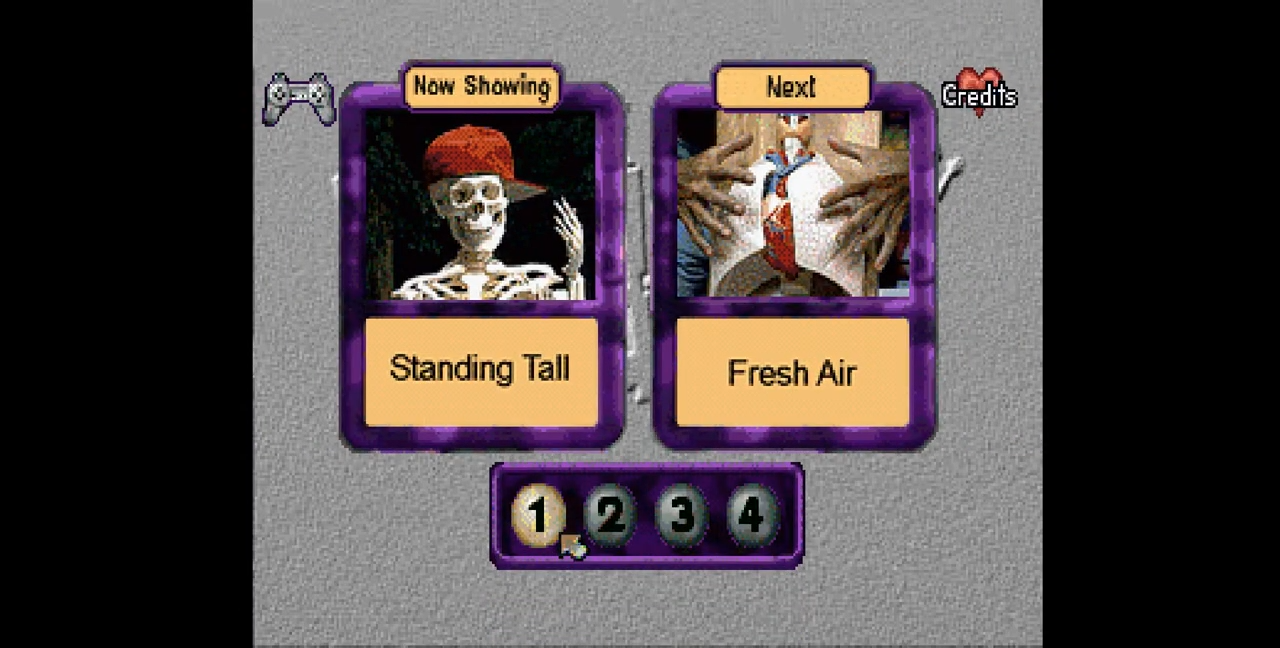
\includegraphics[width=\linewidth]{Games/HeadtoToe/Images/HeadToToe2Image1.png}
        \caption{Head To Toe 2 - Screenshot 1}
    \end{subfigure}
    \begin{subfigure}{0.45\textwidth}
        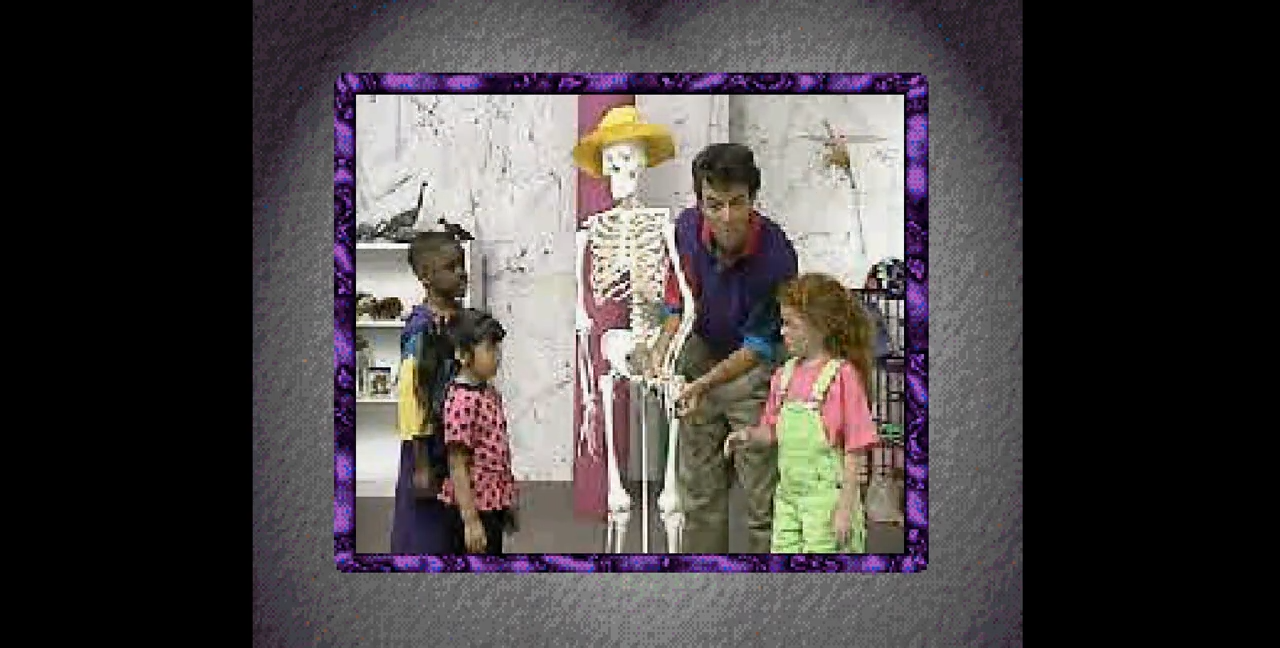
\includegraphics[width=\linewidth]{Games/HeadtoToe/Images/HeadToToe2Image2.png}
        \caption{Head To Toe 2 - Screenshot 2}
    \end{subfigure}

    \begin{subfigure}{0.45\textwidth}
        \centering
        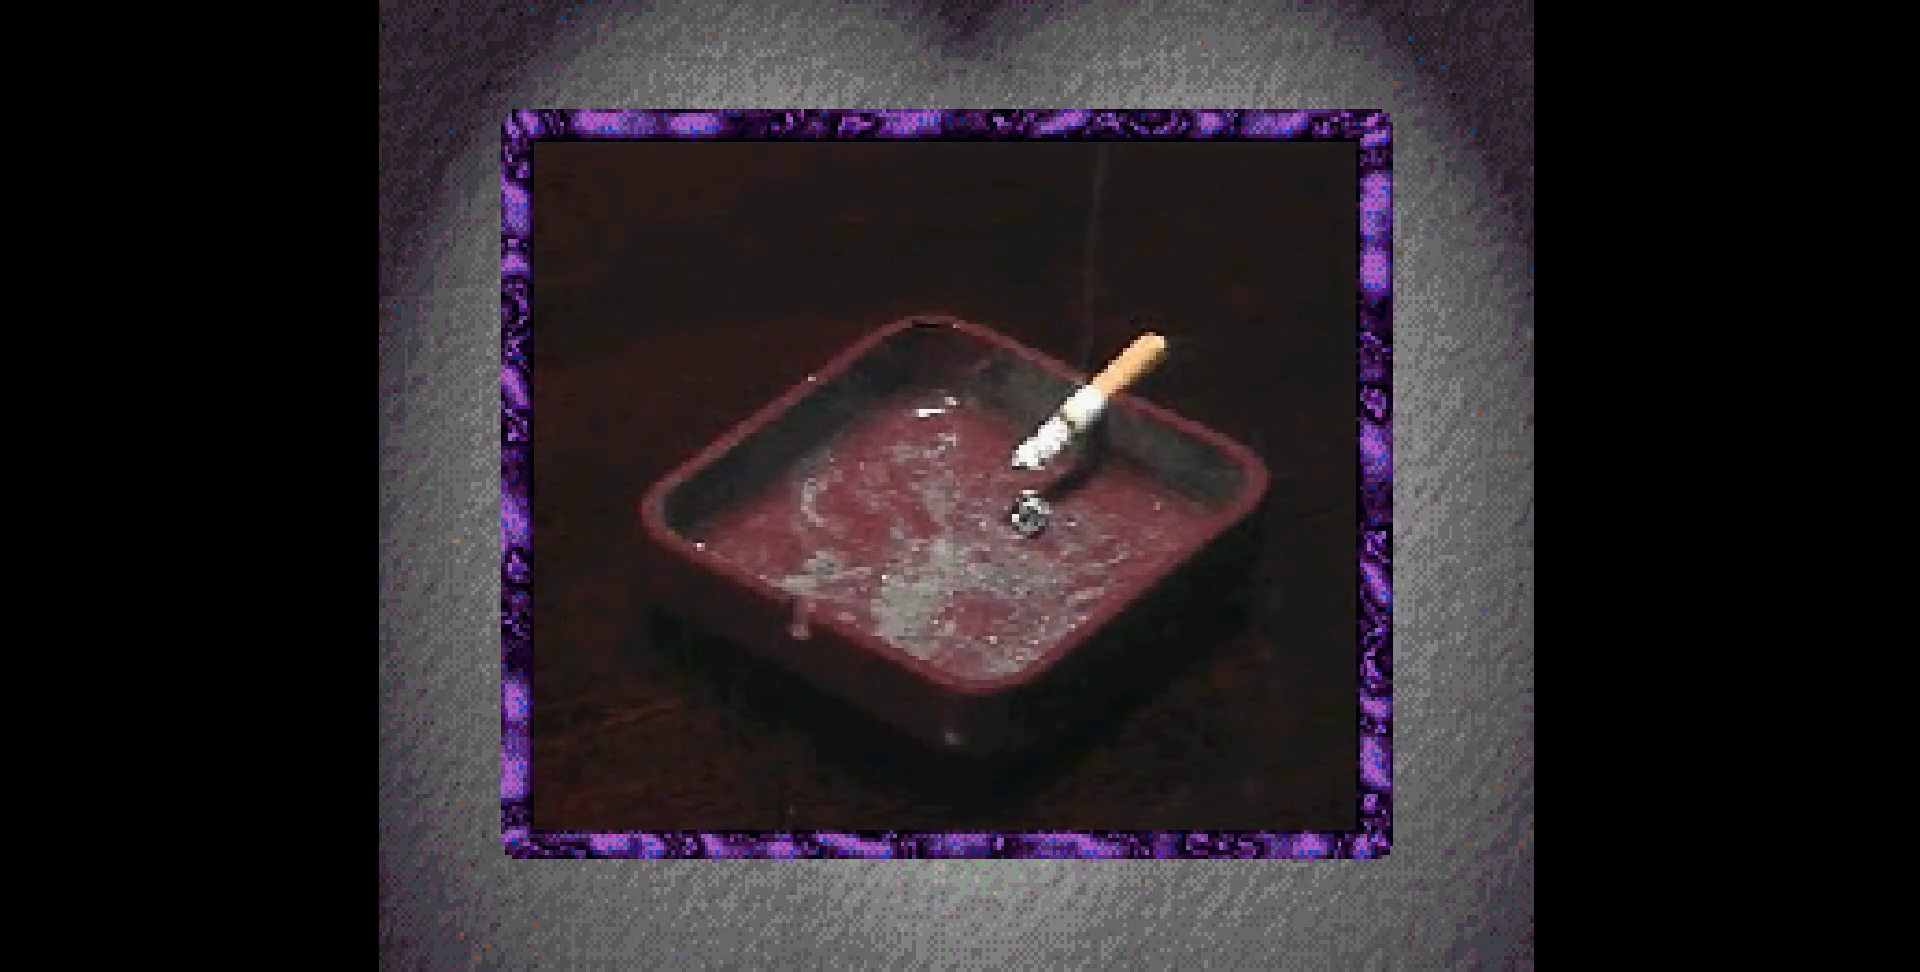
\includegraphics[width=\linewidth]{Games/HeadtoToe/Images/HeadToToe2Image3.png}
        \caption{Head To Toe 2 - Screenshot 3}
    \end{subfigure}
    \begin{subfigure}{0.45\textwidth}
        \centering
        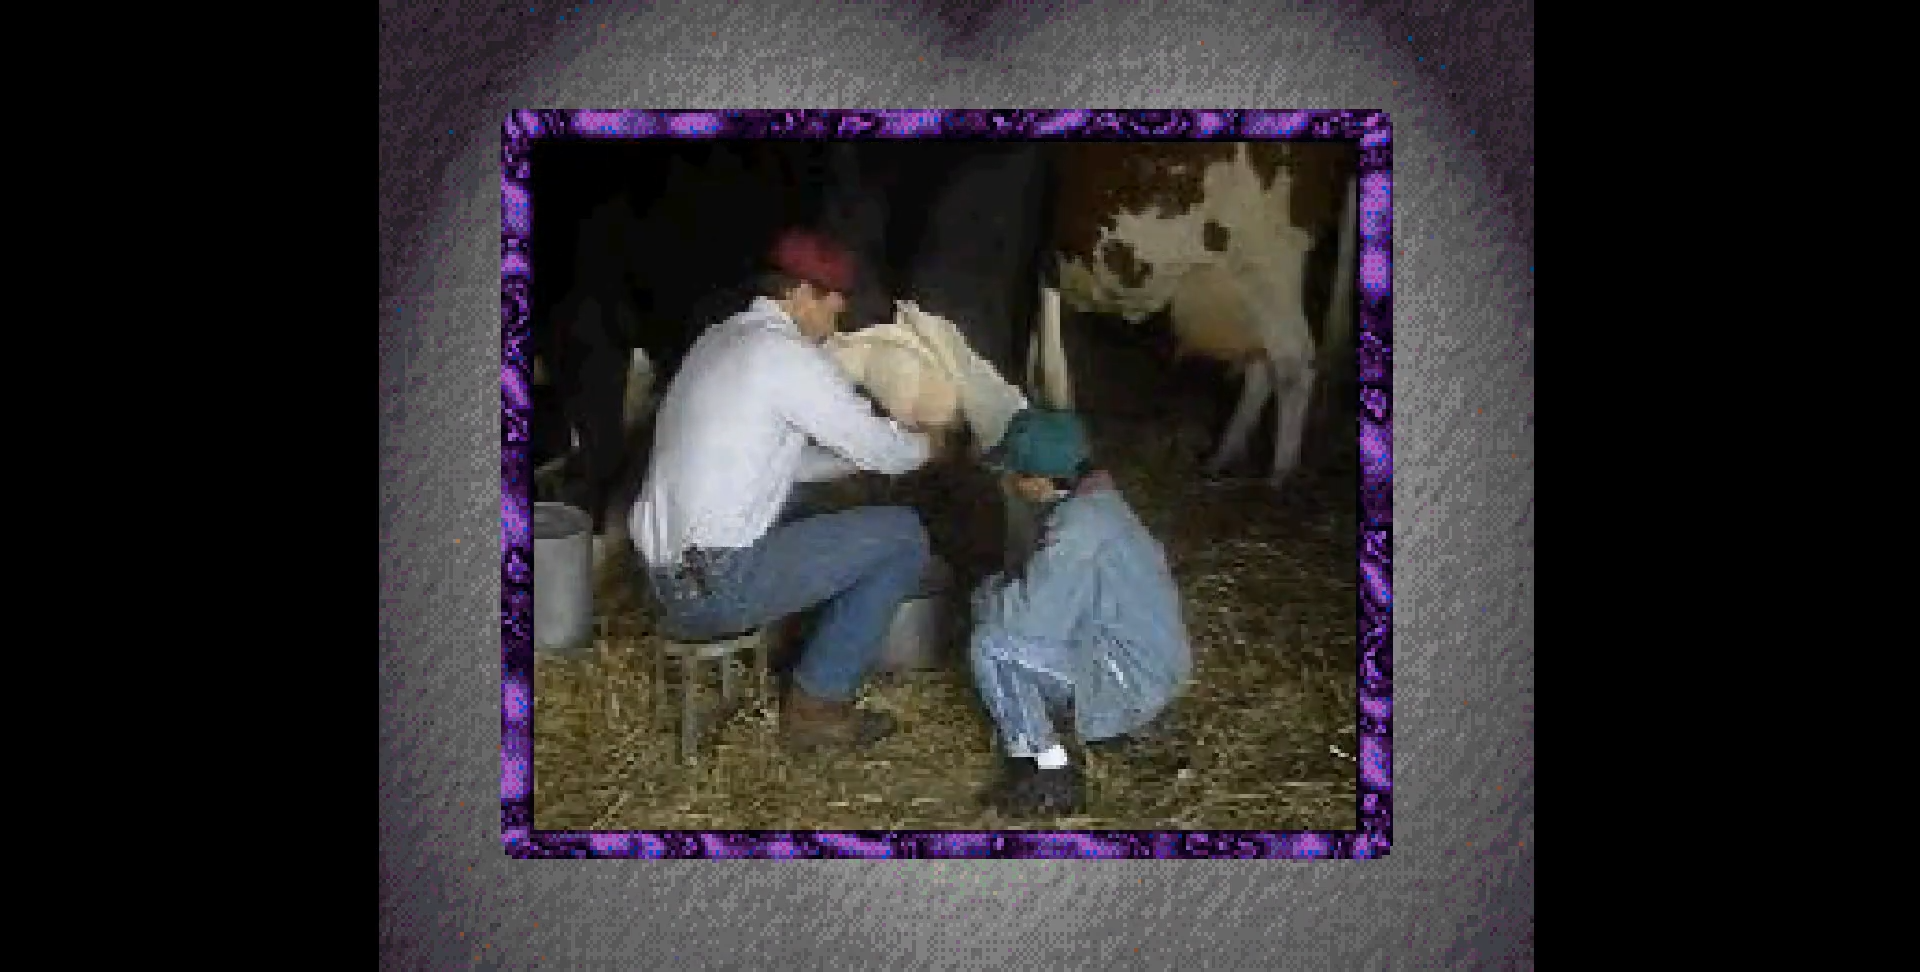
\includegraphics[width=\linewidth]{Games/HeadtoToe/Images/HeadToToe2Image4.png}
        \caption{Head To Toe 2 - Screenshot 4}
    \end{subfigure}
    \caption{Screenshots from Head To Toe 2}
\end{figure}